%%
%% This is file `sample-sigchi-a.tex',
%% generated with the docstrip utility.
%%
%% The original source files were:
%%
%% samples.dtx  (with options: `sigchi-a')
%% 
%% IMPORTANT NOTICE:
%% 
%% For the copyright see the source file.
%% 
%% Any modified versions of this file must be renamed
%% with new filenames distinct from sample-sigchi-a.tex.
%% 
%% For distribution of the original source see the terms
%% for copying and modification in the file samples.dtx.
%% 
%% This generated file may be distributed as long as the
%% original source files, as listed above, are part of the
%% same distribution. (The sources need not necessarily be
%% in the same archive or directory.)
%%
%% The first command in your LaTeX source must be the \documentclass command.
\documentclass[sigchi-a,screen]{acmart}
\usepackage{graphicx}
\graphicspath{ {./images/} }
%%
%% \BibTeX command to typeset BibTeX logo in the docs
\AtBeginDocument{%
  \providecommand\BibTeX{{%
    \normalfont B\kern-0.5em{\scshape i\kern-0.25em b}\kern-0.8em\TeX}}}

%% Rights management information.  This information is sent to you
%% when you complete the rights form.  These commands have SAMPLE
%% values in them; it is your responsibility as an author to replace
%% the commands and values with those provided to you when you
%% complete the rights form.
\copyrightyear{2019}
\acmYear{2019}
\setcopyright{rightsretained}

%% These commands are for a PROCEEDINGS abstract or paper.
\acmConference{CSCW 2019 Workshop - Mapping the How}{November 10, 2019, Austin TX, USA}
% \acmDOI{no DOI}
% \acmISBN{no ISBN}
% \acmBooktitle{No Booktitle}


%%
%% Submission ID.
%% Use this when submitting an article to a sponsored event. You'll
%% receive a unique submission ID from the organizers
%% of the event, and this ID should be used as the parameter to this command.
%%\acmSubmissionID{123-A56-BU3}

%%
%% The majority of ACM publications use numbered citations and
%% references.  The command \citestyle{authoryear} switches to the
%% "author year" style.
%%
%% If you are preparing content for an event
%% sponsored by ACM SIGGRAPH, you must use the "author year" style of
%% citations and references.
%% Uncommenting
%% the next command will enable that style.
%%\citestyle{acmauthoryear}

%%
%% end of the preamble, start of the body of the document source.
\begin{document}

%%
%% The "title" command has an optional parameter,
%% allowing the author to define a "short title" to be used in page headers.
\title[Transition to peer production]{Studying The Process of Transition to Peer Production}

%%
%% The "author" command and its associated commands are used to define
%% the authors and their affiliations.
%% Of note is the shared affiliation of the first two authors, and the
%% "authornote" and "authornotemark" commands
%% used to denote shared contribution to the research.
\author{Johanna Cohoon}
\email{jlcohoon@utexas.edu}
\orcid{0000-0002-3352-9766}
\author{James Howison}
% \authornotemark[1]
\email{jhowison@ischool.utexas.edu}
\orcid{0000-0002-5702-149X}
\author{Cai Fan Du}
\email{cfdu@utexas.edu}
\affiliation{%
  \institution{University of Texas at Austin}
  \streetaddress{1616 Guadalupe Street}
  \city{Austin}
  \state{TX}
  \postcode{78701-1213}
}

%%
%% By default, the full list of authors will be used in the page
%% headers. Often, this list is too long, and will overlap
%% other information printed in the page headers. This command allows
%% the author to define a more concise list
%% of authors' names for this purpose.
\renewcommand{\shortauthors}{Cohoon and Howison}

%%
%% The abstract is a short summary of the work to be presented in the
%% article.
\begin{abstract}
  We are studying \textasciitilde200 scientific software projects that received an NSF SI2 grant to discover whether the projects have achieved sustainability through a transition to open source peer production. The processes we are studying are two: 1) How the projects work (their organizational configuration), and 2) How their way of working has changed over time. Our data is the online presence of the projects (e.g., websites, PDFs, repositories). Our method is to conduct grounded content analysis adopting a persona of a potential contributor to emerge a taxonomy of organizational forms (e.g., peer production, lab group). Projects receive a "start" (e.g., 2011) and "end" (e.g., 2015) organizational form label and a label identifying which specific organization is responsible. A transition is said to occur if either or both of those are different; peer production is said to occur if the "end" organization presents as a peer production community. Challenges include: scaling iterative coding with RAs, visibility of process in websites produced, and incomplete archiving of websites. 
\end{abstract}

%%
%% The code below is generated by the tool at http://dl.acm.org/ccs.cfm.
%% Please copy and paste the code instead of the example below.
%%
\begin{CCSXML}
<ccs2012>
<concept>
<concept_id>10003120.10003130.10011762</concept_id>
<concept_desc>Human-centered computing\textasciitildeEmpirical studies in collaborative and social computing</concept_desc>
<concept_significance>500</concept_significance>
</concept>
</ccs2012>
\end{CCSXML}

\ccsdesc[500]{Human-centered computing\textasciitildeEmpirical studies in collaborative and social computing}

%%
%% Keywords. The author(s) should pick words that accurately describe
%% the work being presented. Separate the keywords with commas.
\keywords{process, practice studies, empirical methods, scientific software, peer production, open source}


%%
%% This command processes the author and affiliation and title
%% information and builds the first part of the formatted document.
\maketitle


\section{The Research}

As software becomes more important to the practice of science, policy makers and scientists are more concerned about a perceived lack of sustainable software produced by grant funded projects. Major funders like the NSF have encouraged the adoption of what practitioners refer to as "the open source way" \cite{howison_collaboration_2014} \cite{red_hat_community_architecture_open_2009} and the academic literature has termed "peer production" \cite{benkler_coases_2002} \cite{von_hippel_open_2003}. Peer production is attractive as a sustainability model because it enables users of the software to collaboratively sustain it and because it draws resources from diverse sources rather than seeking ongoing grants to support maintenance \cite{gambardella_proprietary_2005} \cite{katz_report_2016}. To understand whether and how projects can transition from primarily relying on grant funding to achieving sustainability through open source communities we conducted a qualitative research study.

We studied both the process of software development (how they work) as well as the process of transitioning between sustainability models (how the way they work has changed). We conducted a grounded content analysis of grants funded by the NSF program "Software Infrastructure for Sustained Innovation" (SI2). The NSF SI2 program specifically intends to create "sustainable software communities" and the solicitation instructions specifically require each project to have a "Sustainability Plan" \cite{noauthor_software_2016}.

\section{How we assess process}

Genre theory provides a solid theoretical grounding for what we've seen in the field: that different types of organizations and their processes (or practices) produce different types of documents \cite{yates_genres_1992}. Thus we operationalize the way that projects work by looking at the form and content of the websites they produce.

For each grant, we collected publicly available documents. We began with the published grant abstract located on the NSF website. To locate other relevant documents, we searched the web using keywords like grant numbers, titles, names of software, and names of personnel mentioned on the grants (including any linked collaborative grants). Documents discovered varied for different projects but included project homepages, SI2 PI meeting posters, published papers, PI institutional websites, mailing list archives, and source code repositories (e.g., Github, Sourceforge, Bitbucket). We often discovered new documents by following links from previously discovered websites. For instance, code repositories were frequently discovered because the project homepage linked to them. 

To study the process of change over time, we initially planned a panel study (one observation in \textasciitilde2015, one in \textasciitilde2019) but were stymied by the length of time needed to complete one round of coding. Instead we have relied on web archives accessed through The Wayback Machine, working in 2015 to get all known websites into their archiving schedule. Looking at archives of the same websites throughout the funding period we were able to see how the content and form of the pages changed. 

Because peer production "lives or dies" by the size and activity of its contributor pool \cite[page 3]{pierce_patching_2015}, as we searched for documents we adopted the persona of a potential contributor. Reaching such people would be key to successful establishment of peer production and thus it is reasonable to expect that we would find any successful transitions to peer production by using that persona.

Throughout our analysis, as Corbin and Strauss \cite{corbin_basics_2014} advise, the practices of memo-ing and discussion both recorded and advanced our work. As we were "dialoguing with the data" \cite[page 106]{corbin_basics_2014}, our findings became clearer and more distinctly tied to the organizational and genre studies literatures. We explored organizational science literature for appropriate frameworks to formalize our analysis, finding that organizational configurations \cite{fiss_set-theoretic_2007} \cite{mintzberg_structure_1980} best complimented our approach. Configurations are potential structures that an organization might adopt \cite{mintzberg_structure_1980}, identified by finding resemblances among various organizations \cite{short_research_2008}.

As we discussed project characteristics, we created tables to compare and sort projects (e.g., Table 1, which shows the different modes of scientific software transition identified through our research). Gradually, patterns emerged in our codes. Our notes showed, for example, that some grants created a name for their group while others did not. Furthermore, within those named groups, some had websites promoting the reputation of specific participants while others promoted the software. Some projects presented separately from their grants, while others foregrounded the grant. Some projects explicitly invited contributions, others listed "lab members". Labeling and defining these patterns, we identified four configurations for grant-funded software development. Repeatedly examining each grant, we considered whether their characteristics fit or gave exception to the configurations we defined. This process of "integrating categories and their properties" (Glaser, 1965) refined our definitions and, therefore, our findings. 

\begin{marginfigure}
    \centering
    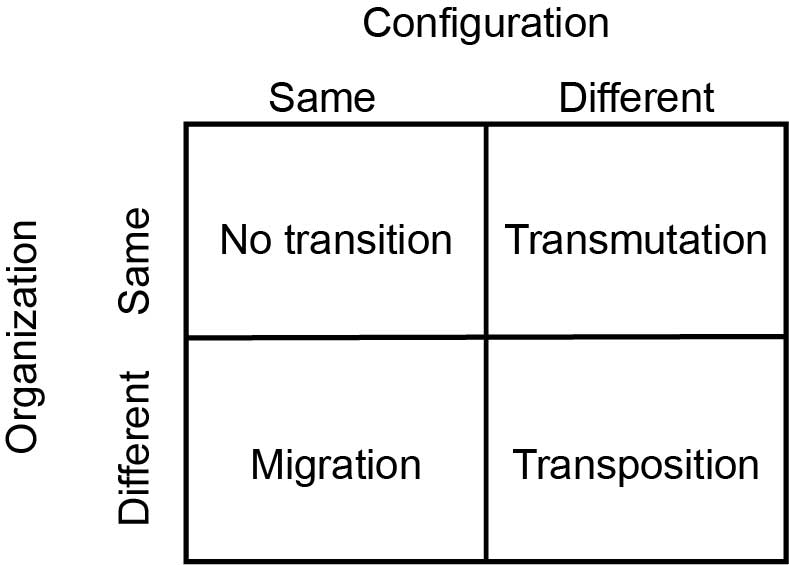
\includegraphics{images/2x2.jpg}
    \caption{Table showing the possible modes of transition. Software can transition by the organization maintaining it changing its own configuration or by the software being passed on to another organization that may, or may not, have a different configuration.}
    \label{fig:table1}
\end{marginfigure}

Following this iterative process of data collection, analysis, and literature review, we grew and repeatedly re-organized our dataset (often having to recode large numbers as new codes emerged). As we saw trends developing or better articulated emergent concepts, we revised our coding scheme. To allow for such revision but still keep a record or our data's provenance, we recorded our work as structured data in RDF and versioned it using git. 

\section{The Challenges}

Here we highlight four challenges we have faced while conducting this research.

The first is visibility of process in artifacts produced. Unlike some trace data studies where the traces are event data (messages posted to a venue, code committed, produces launched), our data are static snapshots of how projects present to the world. While we think we have strong face validity in distinct and recognizable genres of websites, we worry about how well those websites represented projects at any particular moment in time. This is because older websites are not necessarily "cleaned up" and projects migrate their "front doors" without much visible comment. If the projects we examined did not keep their web presence up to date, our inferences about their work processes may be behind the times. 

The second challenge is related: Given that we only examined public documents, the depth of our insight into project organization is necessarily skewed by the openness of the projects. For example, we did not seek to conduct interviews with participants nor attempt observations at project meetings or universities. Thus, projects that were less open tended to have fewer publicly available documents we could examine. Nonetheless, given that these are NSF funded projects intended to create software used by others, all grants produced some documents, even if limited to sources such as SI2 PI meeting posters, institutional homepages of PIs, and published papers. Thankfully, our interest is mostly in peer production or its absence, and we can be confident that we did not miss any projects that established sustainable peer production because peer production is defined by open online presence. 

The third challenge is scaling and interaction. We intentionally sought to undertake a "medium N" sized study \cite{ragin_redesigning_2009} beginning with \textasciitilde200 grants. But the number of documents studied was significantly greater because grants often funded work on multiple software projects, each of which might have multiple websites. We tried to speed up this research process by using undergrad and graduate RAs. As RAs needed to learn both our own data infrastructure and the coding scheme, however, the on-boarding time was significant, updating codes across large groups difficult, and re-coding de-motivating. The iterative and emergent coding approach interacted with the scale, making changes increasingly expensive as our research progressed. For example, we initially coded by grant but had to adjust our unit of analysis from grant to project, re-assigning codes and introducing new ones.

The fourth challenge stems from studying process as change in public presentations. Once we knew of a website we could add it to the Wayback Machine internet archive to monitor change from that time on, but (of course) we couldn't go back further than that. Similarly, if we discovered one later in our process, we simply had to hope that it had been archived. This meant that it was difficult to situate the website content and project work in their original circumstances. For example, by discovering an old blog post, we learned that one software project was forced to temporarily stop development work and change their license because of a lawsuit brought by the former employer of the software's primary author. As a consequence of this lawsuit, for a year and a half the software project was not open source---a dramatic shift from what had been a young peer production community. Without that blog post we might have read the license change "as a rational plan" \cite[page 70]{suchman_human_2007} rather than a response to a change in circumstances. 

As we seek to find a balance between producing valid insights and using sustainable research practices of our own, we have grappled with these four challenges. They have affected who could participate in our research, how we recorded our data, as well as how we can interpret our findings. 

% \section{SIGCHI Extended Abstracts}

% The ``\verb|sigchi-a|'' template style (available only in \LaTeX\ and
% not in Word) produces a landscape-orientation formatted article, with
% a wide left margin. Three environments are available for use with the
% ``\verb|sigchi-a|'' template style, and produce formatted output in
% the margin:
% \begin{itemize}
% \item {\verb|sidebar|}:  Place formatted text in the margin.
% \item {\verb|marginfigure|}: Place a figure in the margin.
% \item {\verb|margintable|}: Place a table in the margin.
% \end{itemize}

%%
%% The acknowledgments section is defined using the "acks" environment
%% (and NOT an unnumbered section). This ensures the proper
%% identification of the section in the article metadata, and the
%% consistent spelling of the heading.
\begin{acks}
This material is based upon work supported by the National Science Foundation under Grant No. 1453548.
\end{acks}

%%
%% The next two lines define the bibliography style to be used, and
%% the bibliography file.

\bibliographystyle{ACM-Reference-Format}
\bibliography{references.bib}

\appendix

\section{Biosketches}

\subsection{Johanna Cohoon}
Johanna (Hannah) Cohoon is a PhD Candidate at the Information School of the University of Texas at Austin where she studies scientific research practices and cyberinfrastructure. Previously, she worked at the Center for Open Science where she researched reproducibility in Psychology. She is interested in how scientific norms and practices change. Johanna received her bachelors degree in Cognitive Science from the University of Virginia. 

\subsection{James Howison}
James Howison is an Associate Professor in the Information School of the University of Texas at Austin, where he has been since August 2011, following a post-doc at CMU and his 2009 PhD from Syracuse Information School. James has studied open source software development and the development of software in science because both are interesting examples of collaboration, and is particularly interested in understanding how different incentives, such as working for fun or for academic reputation, lead to different structures of collaboration. James is a 2019 PECASE award winner, based on a NSF 2014 CAREER award. Publications include MISQ, Information and Organization, and CSCW. \href{http://james.howison.name}{http://james.howison.name}

\subsection{Cai Fan Du}
Fan is a doctoral student at the Information School of the University of Texas at Austin. She is a sociotechnical researcher interested in the organizing of distributed efforts in the production of digital artifacts. 

\end{document}
\endinput
%%
%% End of file `sample-sigchi-a.tex'.
